\chapter{Performance Evaluation} \label{ch:evaluation}

To evaluate the efficiency and flexibility of multiple flow table mechanism, the vCPE service with the proposed mechanism was deployed by the HSNL vCPE framework and two kinds of experiments are organized as follow: multiple table performance evaluation and integration evaluation.
The performance measurement focused on measuring the NAT anf forwarding performance on Virtual CPE.
The integration evaluation was designed for proving the functionality of all network functions of our vCPE, and thus demonstrating the flexibility of our proposed multiple flow table mechanism to integrate with another services.

\section{Multiple Table Performance}

\begin{figure}[!t]
\centering
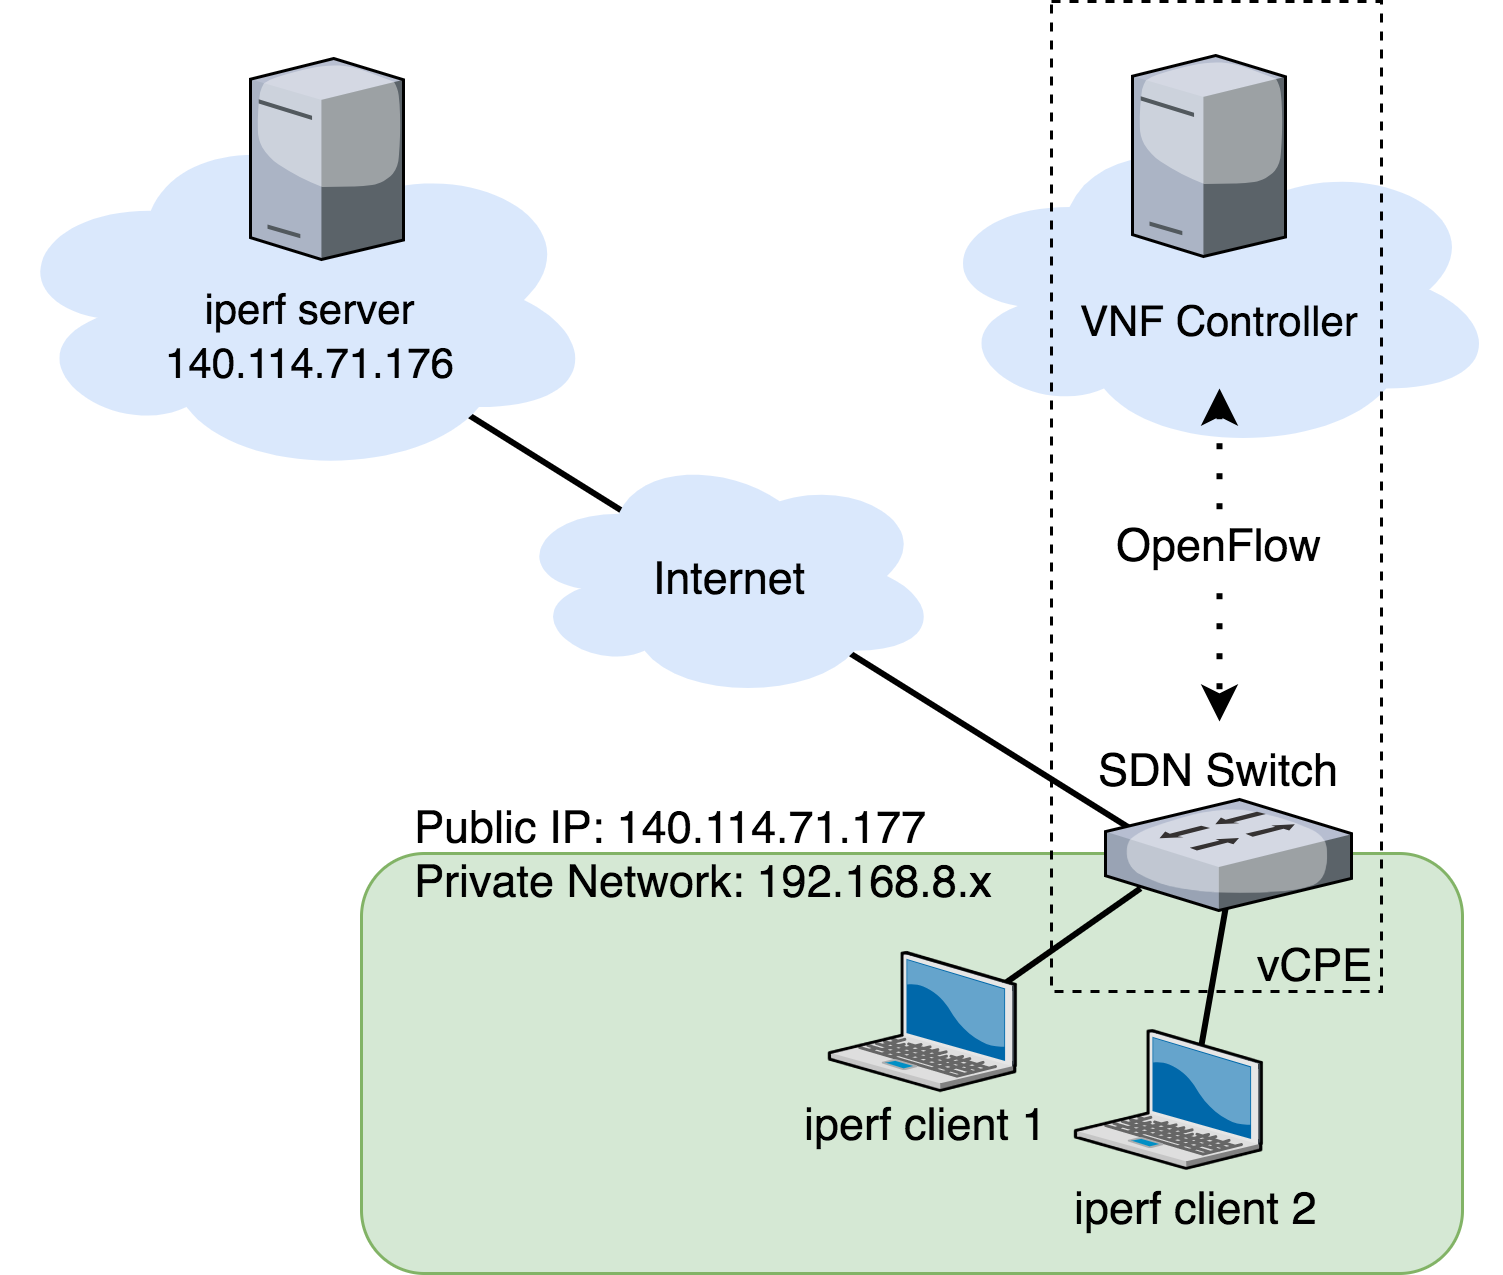
\includegraphics[width=\textwidth]{./fig/throughput_measurement_scenario.png}
\caption{Multiple Table Performance Evaluation Scenario.}
\label{fig:throughput_measurement_scenario}
\end{figure}

Implementing a single flow table framework is easier than implementing a multiple flow table framework; however, multiple flow table frameworks are more flexible.
To verify the efficiency of the multiple flow table vCPE framework, we conducted an experiment by using the NAT and forwarding service to compare the throughput between single flow table vCPE and multiple flow table vCPE.

An overview of the experimental environment is presented in Fig. \ref{fig:throughput_measurement_scenario}.
The NFV controller was run on the Dell PowerEdge R630 rack server, and the EdgeCore AS5712-54X \cite{edge-core-switch} was used as the SDN switch.
We used iPerf \cite{iperf} to generate network traffic.
The iPerf server connected the public IP address with 140.114.71.176, and then the iPerf client connected to the SDN switch and was controlled by the NFV controller.
The NFV controller ran the NAT service, but used different frameworks, a single flow table and multiple flow table.

\begin{figure}[!t]
\centering
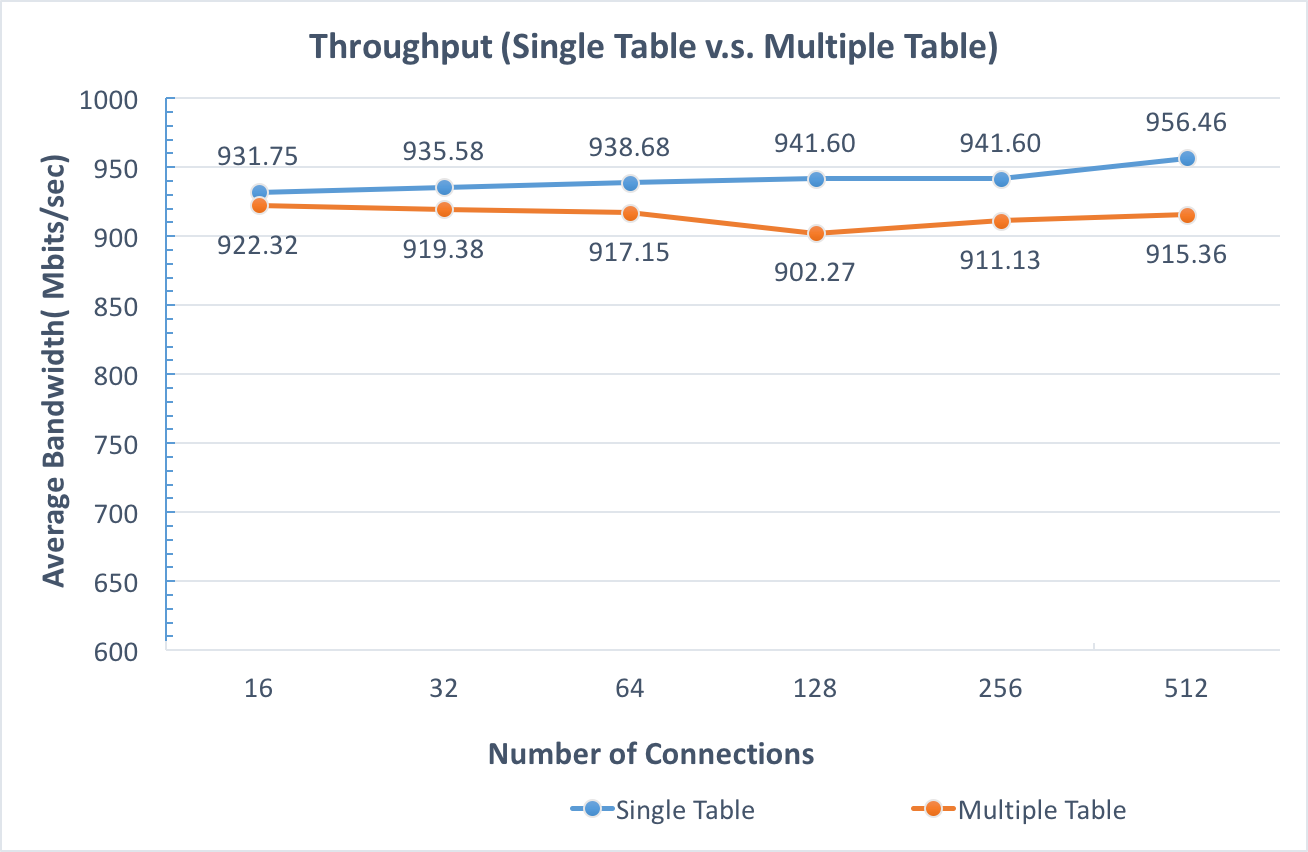
\includegraphics[width=\textwidth]{./fig/throughput_measurement.png}
\caption{Results of Multiple Table Performance Evaluation.}
\label{fig:throughput_measurement}
\end{figure}

We used iPerf to generate TCP packets and send them to the server from the client.
In this experiment, different number of connections were used to evaluate the performance of the flow tables.
As shown in Fig. \ref{fig:throughput_measurement}, the throughput values indicated that the performance for the low number of connections are similar.
But if we increased the number of connections, the difference of performance between the two applications performance become bigger and bigger.

For each connection, the multiple table application added 4 rules and single table application added merely 2 rules. Since the multiple table applications needed more rules than the other, the throughput of the multiple table framework is worse than the throughput of the single table framework for the large number of connections conditions.
Although the value of multiple table framework is lower than single table framework at the more number of connections, the multiple table framework is more flexible in add new services in to our vCPE.


\section{Integration Evaluation}


\subsection{Evaluation of QoS When Host Bandwidth Is Limited}

\begin{figure}[!t]
\centering
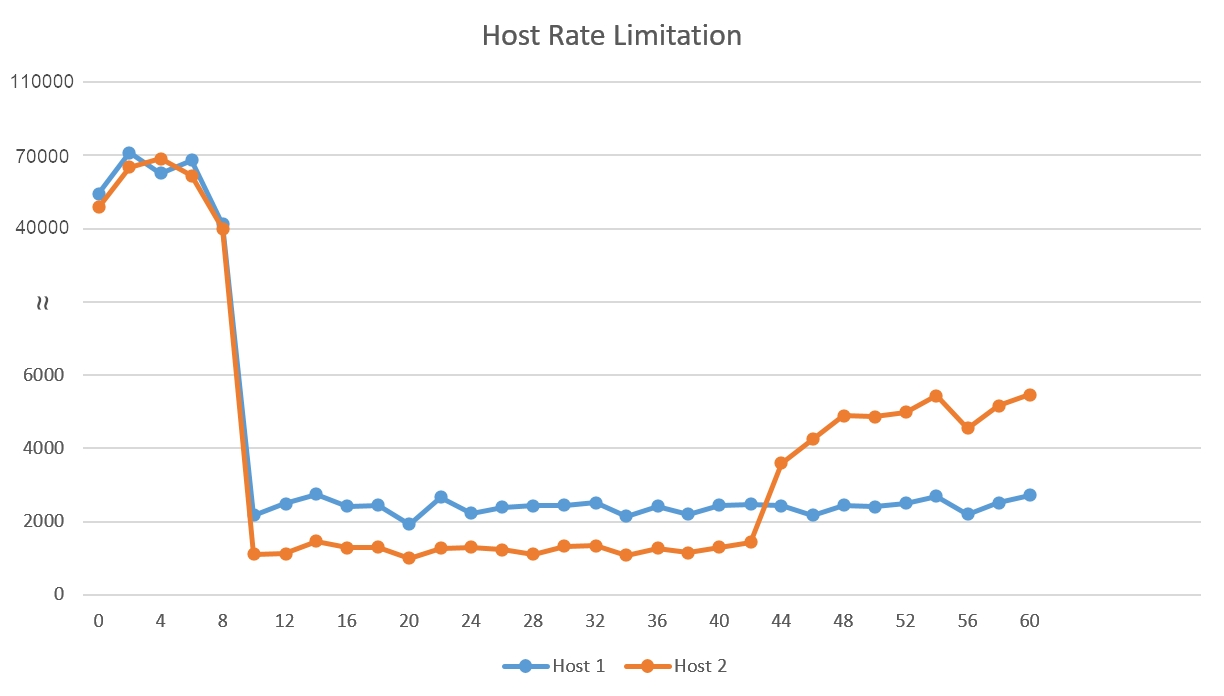
\includegraphics[width=\textwidth]{./fig/integration_host.png}
\caption{Limit the rate of a certain host.}
\label{fig:integration_host}
\end{figure}

Because downloading is a situation that always consumes network resources in practice,
we verify our function by downloading an image of Ubuntu 14.04 that was approximately 1 GB in size.

The NFV controller ran on the Dell PowerEdge R630 rack server and executed QoS.
The Edge-Core AS5712-54X \cite{edge-core-switch} switch was used as the OpenFlow-enabled switch with the PicOS TM r2.6 operating system.
We used a desktop computer as the experimental host to record the bandwidth every 2 seconds.

As shown in Fig. \ref{fig:integration_host}, we started downloading the file without rate limiting and the rate was between 40,000 and 70,000 Kbps.
At the \nth{8} second, we limited the host 1 to 2048 Kbps and host 2 to 1024 Kbps by adding the rule of their MAC address.
Then the bandwidth from host 1 and host 2 is decreasing.
Host 1 and host 2 were limited to approximately 2048 Kbps and 1024 Kbps, respectively.
At the \nth{42} second, we change the bandwidth to host 2.
That is, we set the bandwidth to host 2 from 1024 Kbps to 5120 Kbps.
We observed that the bandwidth of the host 2 rapidly increased to 5120 Kbps.



\subsection{Evaluation of QoS When Application Bandwidth Is Limited}

\begin{figure}[!t]
\centering
\includegraphics[width=0.8\textwidth]{./fig/integration_evaluation.png}
\caption{Scenario of integration evaluation.}
\label{fig:integration_evaluation}
\end{figure}


Our experimental environment is presented in Fig. \ref{fig:integration_evaluation}.
In our experimental environment, we mirror all traffic from the SDN switch to application classification system and identify those flows belong to which application.
Then the application classification system uploaded the classification results to the database.
Subsequently, the controller received the results from the database and updated the flow information of the applications.
Therefore, we could use the flow information (5-tuple and classification results) to limit the application bandwidth.

We selected FileZilla to verify our function for limiting applications and there are two hosts (host 1 and host 2) in the same network domain.
Then we limited the bandwidth of FileZilla in this network domain.
That is, the sum of bandwidths from host 1 and host 2.

\begin{figure}[!t]
\centering
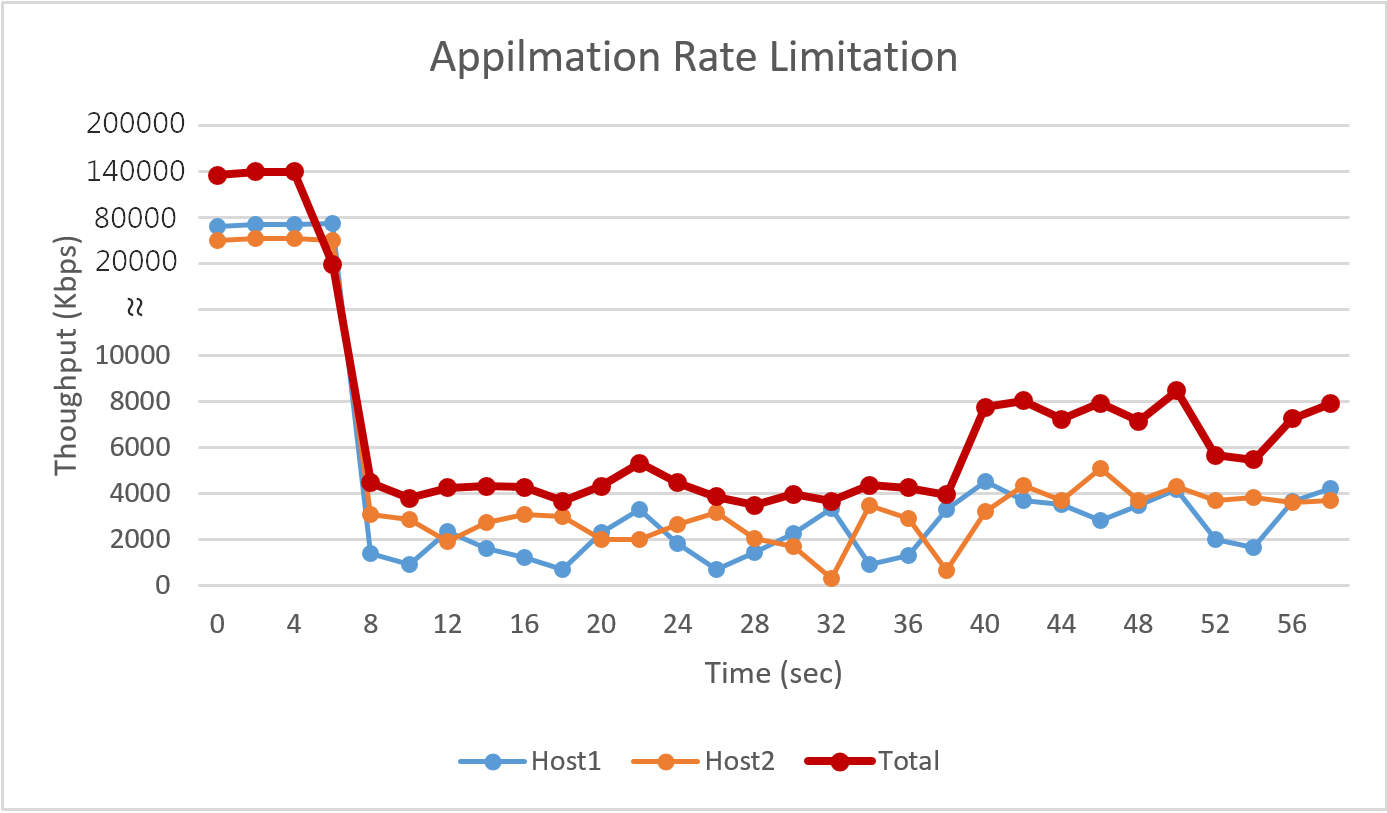
\includegraphics[width=\textwidth]{./fig/integration_app_filezilla.png}
\caption{Limit the rate of Filezilla.}
\label{fig:integration_app_filezilla}
\end{figure}

As shown in Fig. \ref{fig:integration_app_filezilla}.
Initially, without limitation, the total bandwidth of FileZilla was approximately 140000 Kbps.
At the \nth{6} second, we limited the total bandwidth from FileZilla to 4096 Kbps.
Then we observed that the total traffic from FileZilla in this network domain immediately decreased.
Clearly, the total traffic from FileZilla was approximately 4096 Kbps.
At the \nth{38} second, we change the limitation from 4096 Kbps to 8192 Kbps and the total traffic from FileZilla increase to 8192 Kbps as expected.

Using this function for limiting applications, we can guarantee that the traffic in a network domain does not exceed the network capacity, thus preventing traffic congestion.
